\documentclass[11pt,a4paper]{article}

\usepackage[utf8]{inputenc}
\usepackage[T1]{fontenc}
\usepackage[english]{babel}
\usepackage{amsmath,amssymb}
\usepackage[margin=2.5cm]{geometry}
\usepackage{graphicx}
\usepackage{booktabs}
\usepackage{xcolor}
\usepackage[most]{tcolorbox}
\usepackage[colorlinks=true,allcolors=blue!60!black]{hyperref}

\graphicspath{{../output/}}

\definecolor{navy}{HTML}{1F4E79}

% Question statement
\newtcolorbox{question}{
  colback=navy!4, colframe=navy, boxrule=0.6pt, arc=2pt,
  left=6pt, right=6pt, top=6pt, bottom=6pt,
  title=\textbf{Question}
}

% Short factual note: where the data comes from, what the code does
\newcommand{\note}[2]{\smallskip\noindent\textbf{#1.} #2\par}

% Space to write the answer
\newcommand{\answerspace}[1][6cm]{%
  \smallskip\noindent\textbf{Answer}\par\vspace{2mm}%
  \noindent\rule{\textwidth}{0.4pt}\vspace{#1}\par}

\title{Open Macroeconomics \\ \large Mini-tasks and Exam}
\author{Celso Nozema \and Esthevão Marttioly \and Mario Filho \and Victor Lucas}
\date{MSc Economics, FGV EESP \\ Professor: Carlos Eduardo}

\begin{document}
\maketitle

\noindent
Code in \texttt{code/}. Data built by \texttt{code/00\_data.R}, results by
\texttt{code/main.R}. Dynare files in \texttt{dynare/}.
The cycle is Hamilton (2018), $h=2$, $p=2$, throughout.

\tableofcontents
\newpage


%---------------------------------------------------------------
\section{Interest Rates and External Debt}

\begin{question}
Estimate a panel with annual WEO data:
\[ r_{i,t} = \beta_0 + \beta_1 d_{i,t-1}, \]
or, as an extra,
\[ r_{i,t} = \beta_0 + \beta_1 \left( e^{d_{i,t-1} - \bar d_i} - 1 \right), \]
where $d_{i,t}$ is external debt and $r_{i,t}$ the long-run real interest rate.
Two panels: emerging and developed.
\end{question}

\note{Data}{IMF WEO.}
\note{Note}{WEO has no interest rate series, and its external debt block covers
only six regional aggregates. The country-level debt variable is general
government gross debt.}

\answerspace[8cm]


%---------------------------------------------------------------
\section{GDP and Trade Balance}

\begin{question}
Calculate $\mathrm{Cor}(y - y_{pot},\, tb)$ with Brazilian annual data, where
$y - y_{pot}$ is the cycle from a filter of your choice.

\smallskip
\textbf{Extra.} Build $\sigma_y^{BR} / \sigma_y^{US}$, gap volatility, since 1800.
\end{question}

\note{Data}{Brazil 1960 onward: IBGE national accounts, republished by the
World Bank. SIDRA only serves the quarterly system from 1996, so the older
IBGE annual data is reached through WDI. Long series: Maddison Project 2023.}

\note{Method}{Only $y$ is detrended. $tb/y$ is a current-price ratio, already
stationary, so it enters raw. For the extra, both countries are detrended with
Hamilton and the standard deviation is rolled over 30 years, right aligned.
Maddison has Brazil at 1800 and 1820 as isolated benchmark years and annual
data only from 1850, so the series cannot start in 1800. The script prints the
year it actually starts.}

\subsection*{Results}

\[ \rho(tb/y,\ y - y_{pot}) = -0.034 \qquad \text{Brazil, 1963 to 2025} \]

\begin{figure}[h]\centering
  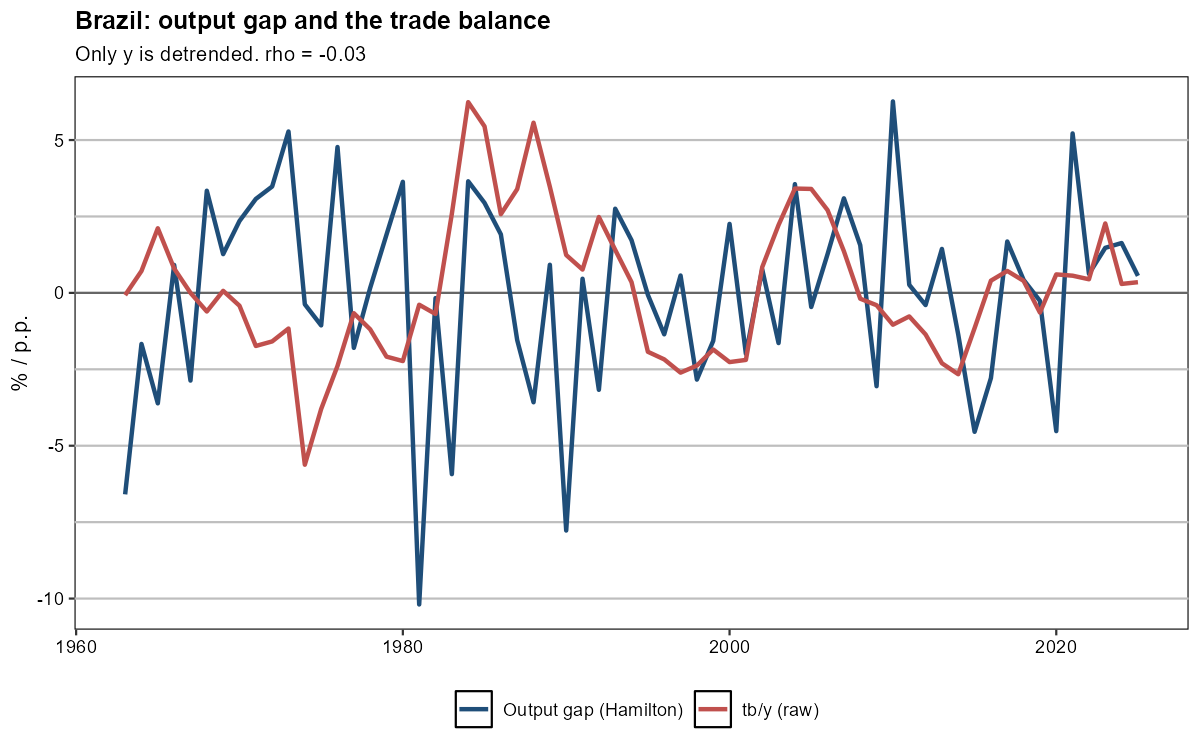
\includegraphics[width=0.8\textwidth]{q2_gap_vs_tb.png}
  \caption{Output gap and the trade balance.}
\end{figure}

\begin{figure}[h]\centering
  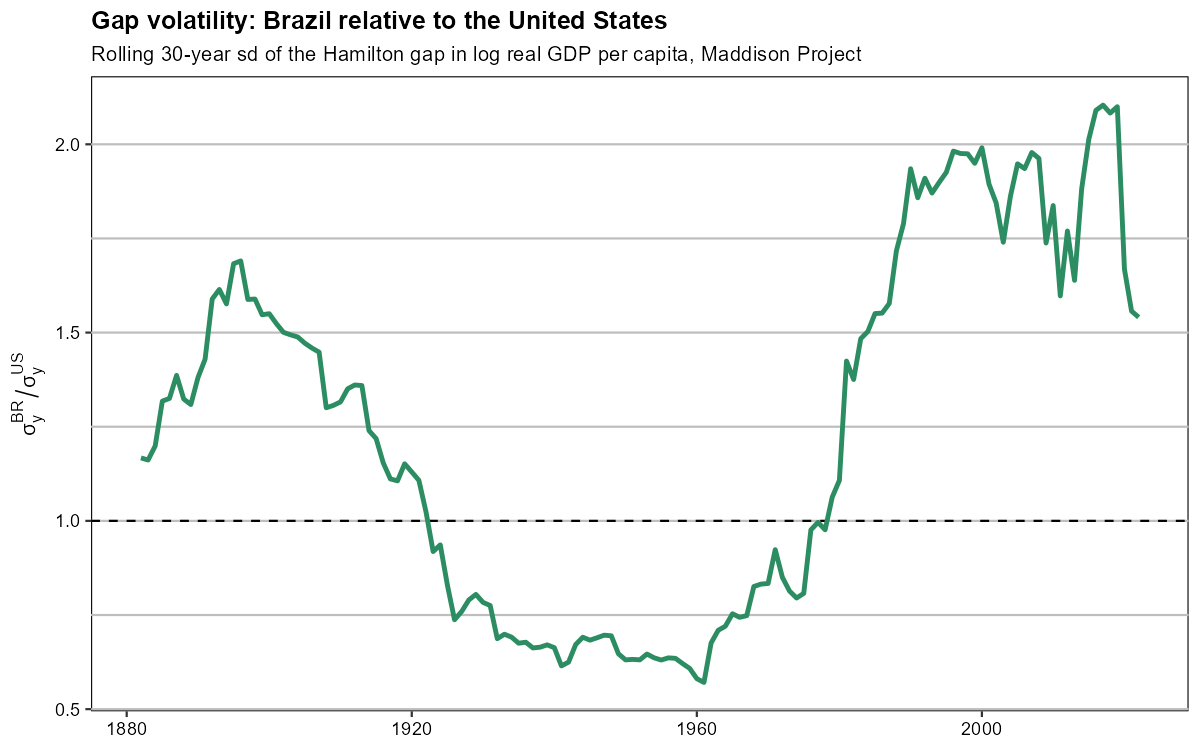
\includegraphics[width=0.8\textwidth]{q2_sigma_br_us.png}
  \caption{Gap volatility, Brazil relative to the United States.}
\end{figure}

\subsection*{Interpretation}

The correlation is $-0.034$, essentially zero. Brazil does not show the
countercyclical trade balance the deck reports for emerging markets, $-0.51$.
This matches Aguiar and Gopinath's $0.01$, and it survives a 62 year sample, so
it is not a short-sample accident.

The figure shows why the number is small. The two series clearly move together
in some decades, the 1980s especially, and against each other in others.

$\sigma_y^{BR}/\sigma_y^{US}$ averages 1.24 over 1882 to 2022, but the swing
matters more than the mean. Brazil is 1.5 times more volatile before 1920, then
falls below the US from 1920 to about 1975, bottoming at 0.57 in 1961. It rises
sharply after 1980 and peaks at 2.10 in 2017. The recent gap is not Brazil
becoming noisier by historical standards. It is the US becoming quieter.


%---------------------------------------------------------------
\section{Sigma Ratios}

\begin{question}
Build the rolling 30-year window for $\sigma_c / \sigma_y$ and compare it to
the rolling 20-year window in the slides.
\end{question}

\note{Data}{Brazil, real per capita GDP and household consumption, 1960 onward.
Same source as Question 2.}

\note{Method}{Both series in logs, detrended once on the full sample. The
window moves the standard deviation, not the trend. Right aligned: the value at
$t$ uses $t-w+1, \dots, t$.}

\note{Note}{The slides use HP(100) and we use Hamilton, which keeps the medium
frequencies HP sends to the trend. Levels here sit above the slides. Table 7 of
the deck shows the same gap.}

\subsection*{Results}

\begin{table}[h]\centering
\begin{tabular}{lcccc}
\toprule
Window & Sample & First & Peak & Last \\
\midrule
20 years & 1982--2025 & 2.13 & 2.28 & 1.08 \\
30 years & 1992--2025 & 1.95 & 2.05 & 1.12 \\
\bottomrule
\end{tabular}
\caption{Rolling $\sigma_C/\sigma_Y$, Brazil.}
\end{table}

\begin{figure}[h]\centering
  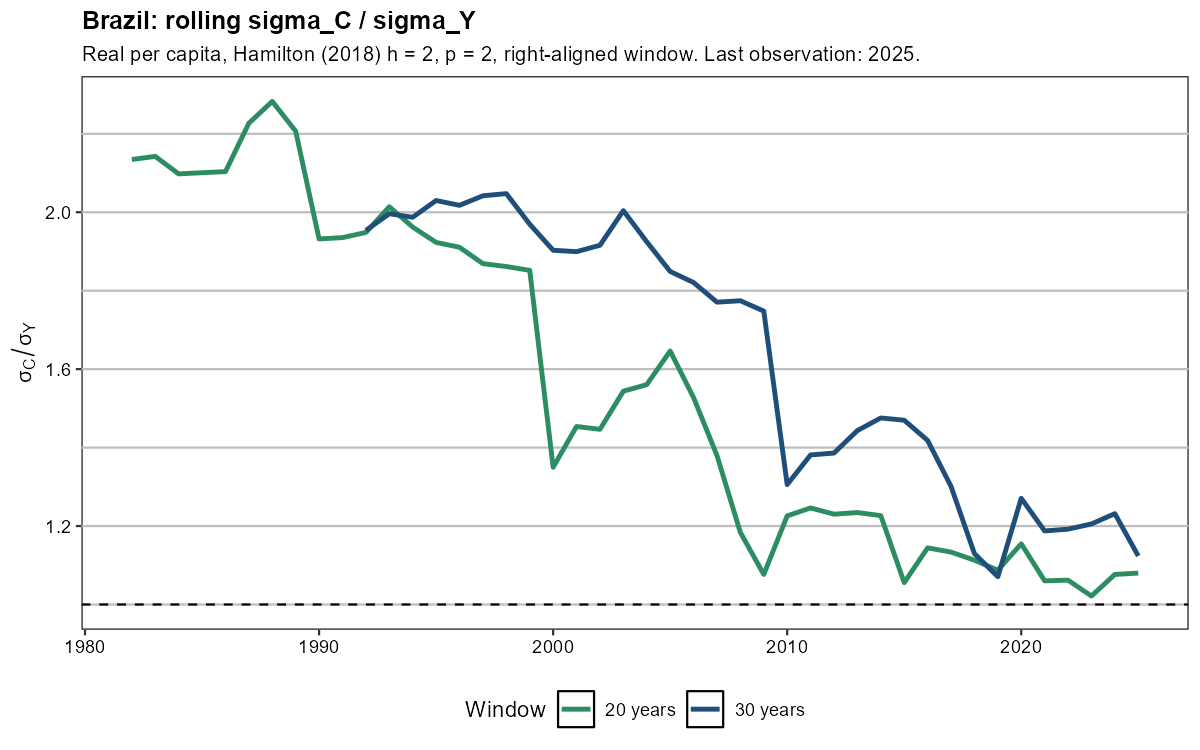
\includegraphics[width=0.8\textwidth]{q3_sigma_ratio_rolling.png}
  \caption{Rolling $\sigma_C/\sigma_Y$, 20 and 30 year windows.}
\end{figure}

\subsection*{Interpretation}

Both windows tell the same story: the ratio was above 2 in the 1980s and 1990s
and is now near 1.1. Brazil's excess consumption volatility has largely
disappeared.

The 30 year window is smoother and lags the 20 year one. It starts ten years
later, and its 2009 drop is the same event the 20 year window recorded in 1999,
the end of the high inflation years leaving the sample. A longer window is not
a better estimate of the same object. It is a slower one.

The two lines converge after 2015 and end together near 1.1. When the window
stops spanning a regime change, the choice of length stops mattering.


%---------------------------------------------------------------
\section{Exchange Rate Volatility vs Trade Volume}

\begin{question}
Compare $\sigma_{ER}$ and $(X+M)/Y$ across countries. Is there more exchange
rate variation in more closed countries?
\end{question}

\note{Data}{World Bank, roughly 200 countries, 1990 to 2024. Official exchange
rate in local currency per US dollar, and trade as a share of GDP.}

\note{Method}{One observation per country. $\sigma_{ER}$ is the standard
deviation of the annual change in $\log$(LCU per USD), openness is the mean of
$(X+M)/Y$. The United States is dropped, being the numeraire. $\sigma_{ER}$ is
right skewed, so the regression is in logs and a Spearman rank correlation goes
beside it. The same correlation is computed within income group, to check the
result is not just rich against poor.}

\subsection*{Results}

\[ \log \sigma_{ER} = a - 0.770 \, \log(\text{openness}), \qquad
   R^2 = 0.046, \qquad n = 151 \]
\[ \text{Spearman} = -0.132 \]

\begin{table}[h]\centering
\begin{tabular}{lcc}
\toprule
Income group & $n$ & Spearman \\
\midrule
High income         & 53 & $-0.089$ \\
Upper middle income & 41 & $-0.277$ \\
Lower middle income & 38 & $+0.116$ \\
Low income          & 18 & $+0.150$ \\
\bottomrule
\end{tabular}
\caption{Correlation of $\sigma_{ER}$ with openness, within income group.}
\end{table}

\begin{figure}[h]\centering
  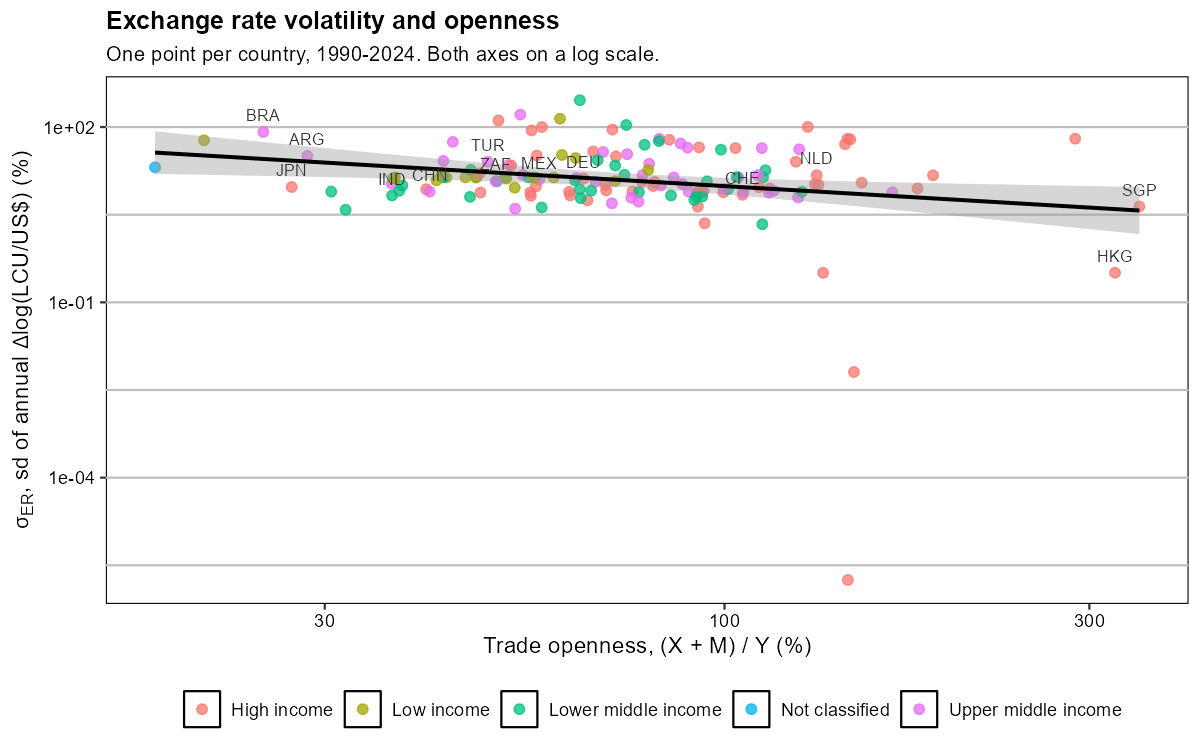
\includegraphics[width=0.85\textwidth]{q4_er_vs_openness.png}
  \caption{Exchange rate volatility against openness.}
\end{figure}

\subsection*{Interpretation}

The slope is negative, so more closed countries do have more exchange rate
variation. But $R^2 = 0.046$ and Spearman $= -0.13$, so openness explains
almost nothing. The cloud in the figure is close to flat.

The sign is not stable across groups either. It is negative for high and upper
middle income countries, positive for the two poorer groups. That is enough to
say the pattern is not a law.

A better reading of the figure is that the outliers do the work. Singapore and
Hong Kong sit far right with low volatility, Brazil and Argentina far left with
high volatility. What separates them is the exchange rate regime, not the trade
share. Hong Kong is pegged and open. Both facts are choices, and openness is
not causing the peg.


%---------------------------------------------------------------
\section{GDP as an AR(1)}

\begin{question}
Estimate
\[ \Delta y_t = \rho\, \Delta y_{t-1} + \varepsilon_t \]
with annual and quarterly Brazilian data.
\end{question}

\note{Data}{Annual: real GDP, 1960 onward, same source as Question 2.
Quarterly: IBGE chained volume index, seasonally adjusted, from BCB SGS 22109,
1996 onward.}

\note{Method}{A constant is included. Brazilian growth has a positive mean and
omitting the constant pushes $\rho$ up to absorb it. The quarterly regression
needs the seasonally adjusted series, since the raw SIDRA index would measure
seasonality instead of persistence.}

\note{Note}{The table also reports $(1+r)/(1+r-\rho)$, the permanent-income
prediction for $\sigma_C/\sigma_Y$ when growth is an AR(1). Comparing it to the
measured ratio in Question 3 says whether the income process alone explains
Brazil's excess consumption volatility.}

\subsection*{Results}

\begin{table}[h]\centering
\begin{tabular}{lccccc}
\toprule
Sample & $\rho$ & s.e. & $t$ & $n$ & $(1+r)/(1+r-\rho)$ \\
\midrule
Annual, 1961--2025      & 0.496 & 0.109 & 4.55 & 64  & 1.91 \\
Quarterly SA, 1996--2025 & 0.049 & 0.092 & 0.53 & 119 & 1.05 \\
\bottomrule
\end{tabular}
\caption{$\Delta y_t = \alpha + \rho \Delta y_{t-1} + \varepsilon_t$.
Implied ratio uses $r = 0.04$.}
\end{table}

\begin{figure}[h]\centering
  
\includegraphics[width=0.8\textwidth]{q5_growth_acf.png}
  \caption{Autocorrelation of GDP growth.}
\end{figure}

\subsection*{Interpretation}

Annual growth is strongly persistent, $\rho = 0.50$ with $t = 4.6$. Quarterly
growth is not, $\rho = 0.05$ with $t = 0.5$, indistinguishable from zero.

The two are not in conflict. They are different samples and different
frequencies. The quarterly series starts in 1996 and misses the high inflation
years, which is where most of the annual persistence comes from.

The annual autocorrelation function decays from 0.50 but not geometrically. It
flattens near 0.20 from order 4 and turns up at order 7. An AR(1) cannot do
that, so the specification is a simplification.

The implied $\sigma_C/\sigma_Y$ from the annual $\rho$ is 1.91, against the 1.08
measured in Question 3 for the recent window and above 2 for the 1980s. The
model matches the old Brazil, not the current one. Note the caveat: $r = 0.04$
is annual, so the quarterly row's implied ratio is not on a comparable footing.


%---------------------------------------------------------------
\section{External Debt Calibration}

\begin{question}
For each emerging country, compare the steady-state external debt $\bar d$
calibrated from $\bar{tb} = r \bar d$ with the actual $\bar d$, the average over
all history. Compute $r$ and $\bar{tb}$ as averages of the available data.
\end{question}

\note{Data}{IMF WEO.}

\answerspace[8cm]


%---------------------------------------------------------------
\section{Hump Shape in Capital}

\begin{question}
Change the Dynare code so that capital responds with a hump shape. Raise the
adjustment cost or the persistence.
\end{question}

\note{File}{\texttt{dynare/q7\_capital\_hump.mod}, from \texttt{soe1.mod}. The
model, steady state and shocks blocks are unchanged. Parameters are set inside
a loop with \texttt{set\_param\_value}, so the calibration in the file is still
the original.}

\note{Method}{The adjustment cost is $\frac{\phi}{2}(k_t - k_{t-1})^2$. With
$\phi$ near zero, as shipped, the firm jumps to the new capital stock in the
period of the shock. Raise $\phi$ and it is cheaper to spread the same
investment over several periods, so capital keeps climbing while TFP is still
high. The interior peak is the hump. Raising $\rho_A$ does the same from the
other side. The file loops $\phi \in \{0.01, 0.5, 2, 6\}$ and
$\rho_A \in \{0.4, 0.7, 0.9, 0.95\}$ and prints the peak period of each.}

\subsection*{Results}

\begin{figure}[h]\centering
  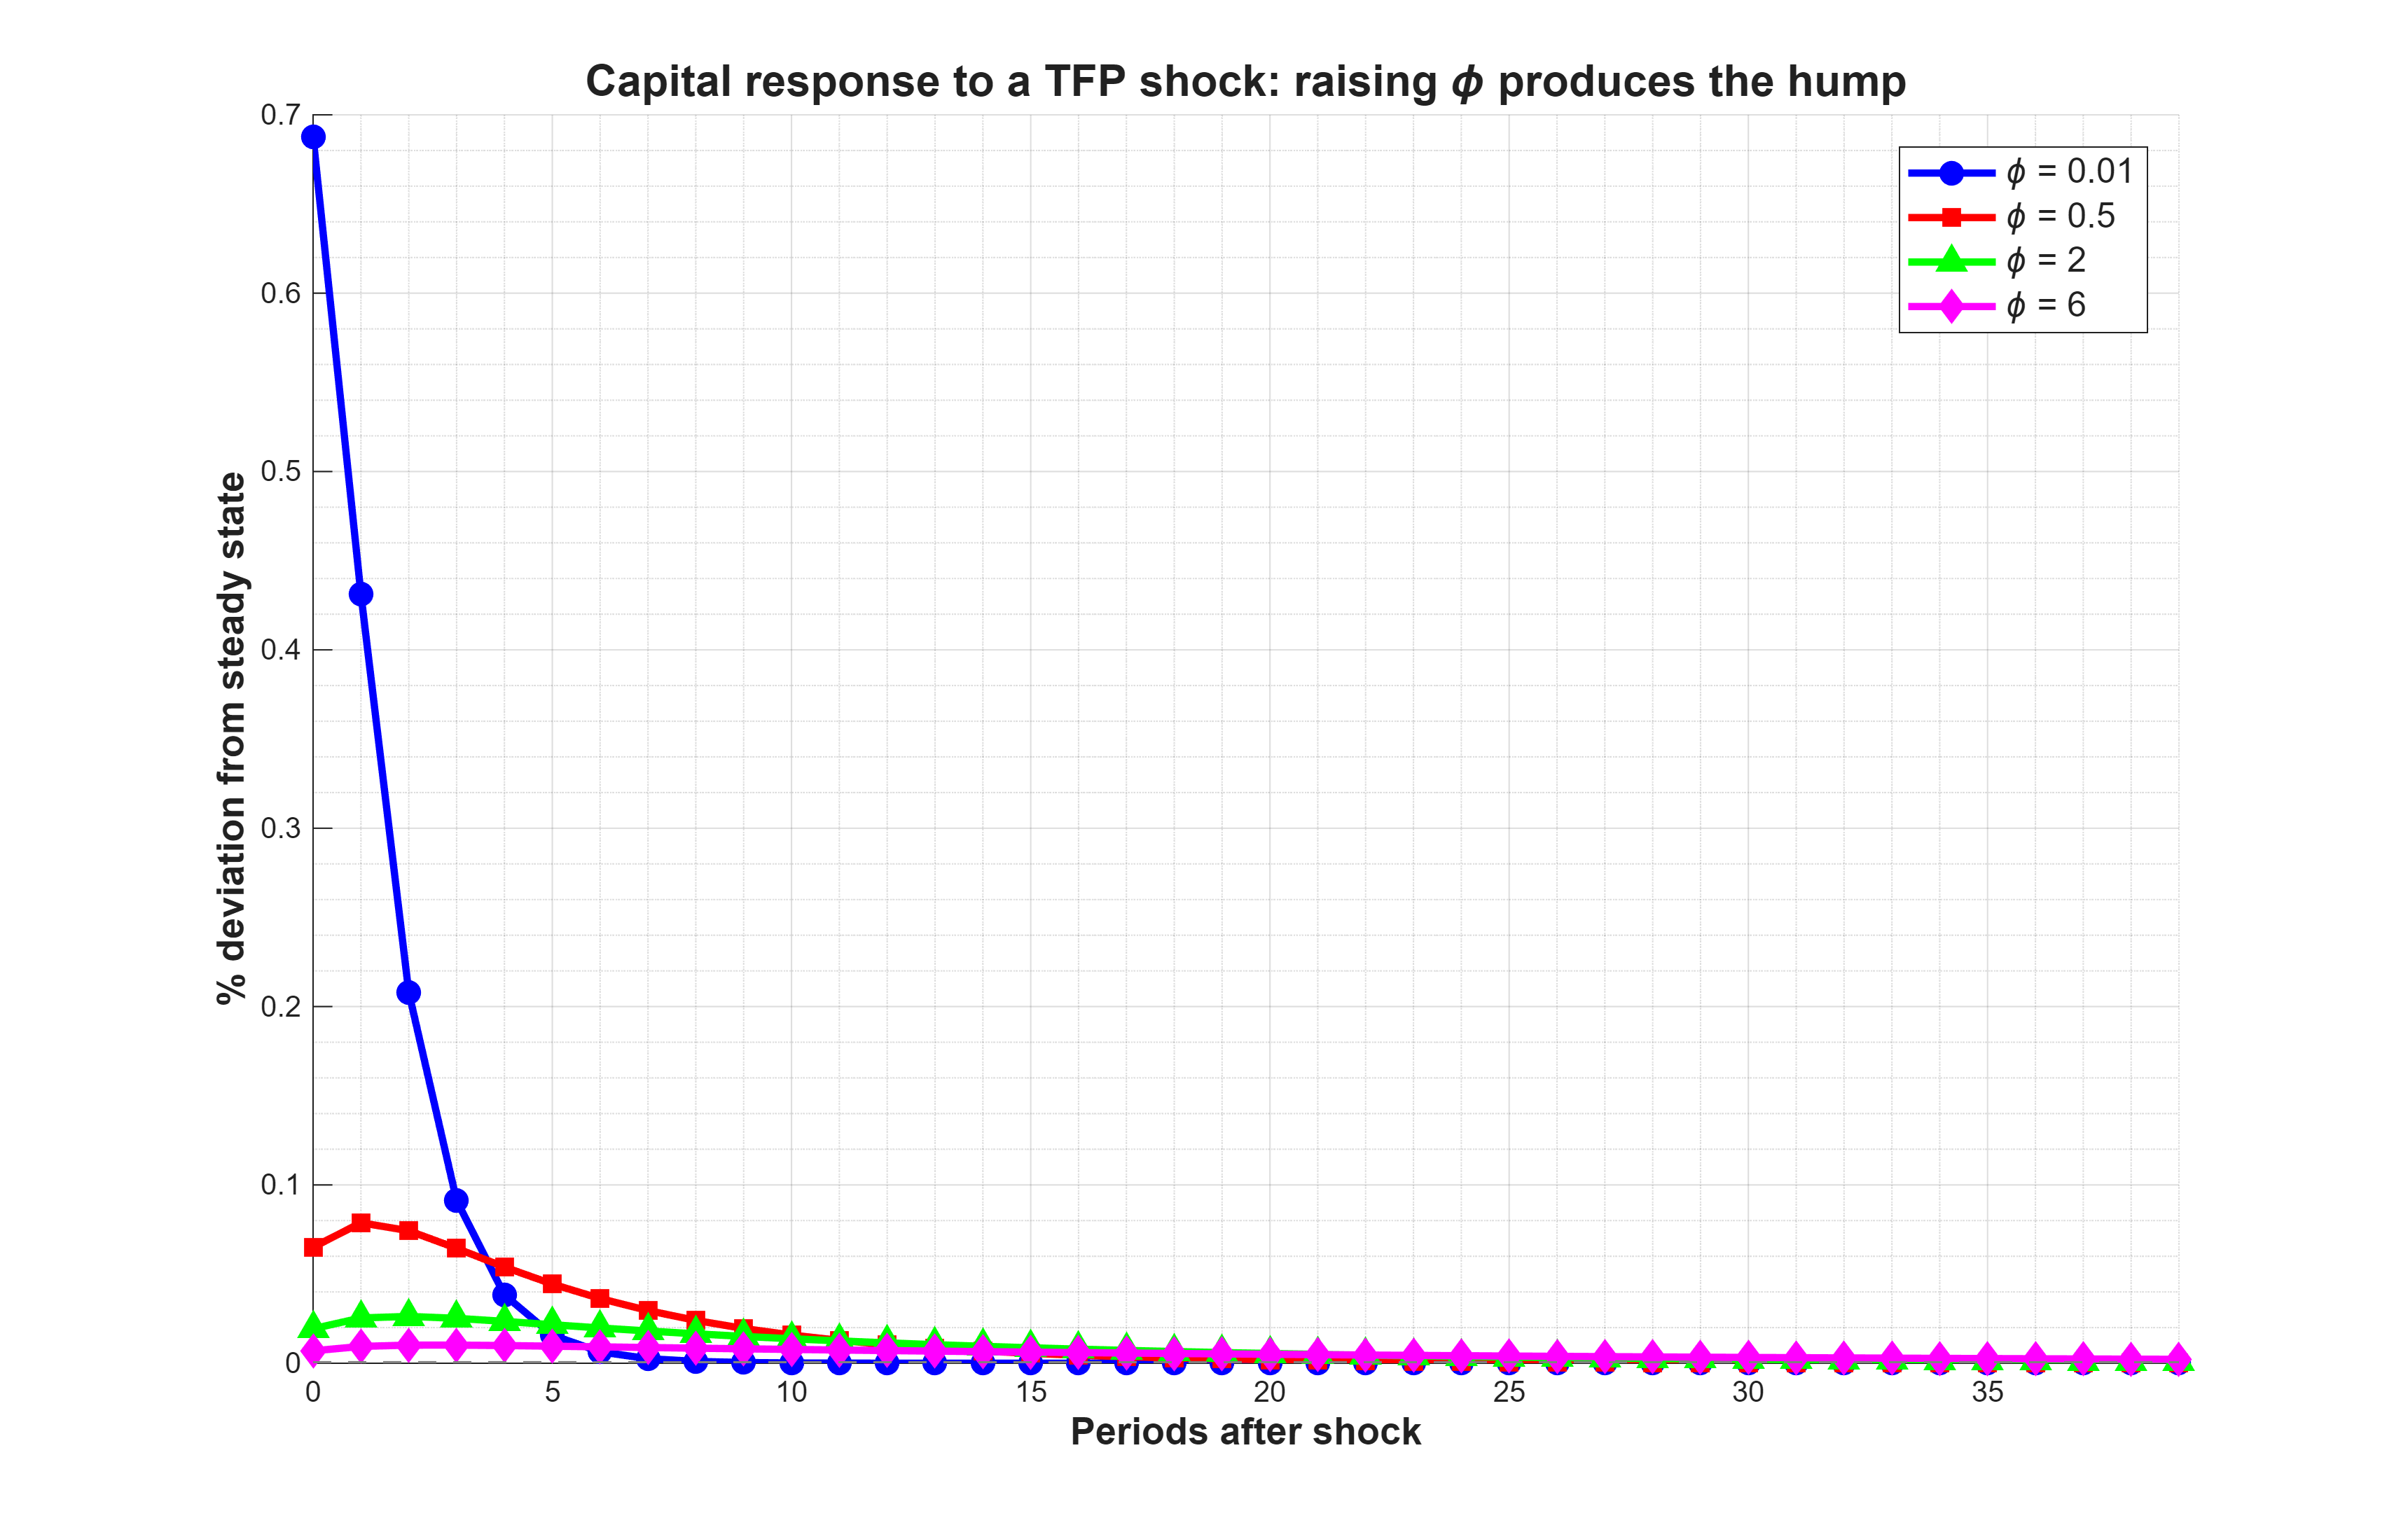
\includegraphics[width=0.78\textwidth]{q7_capital_hump.png}
  \caption{Capital response to a TFP shock, by adjustment cost.}
\end{figure}

\begin{figure}[h]\centering
  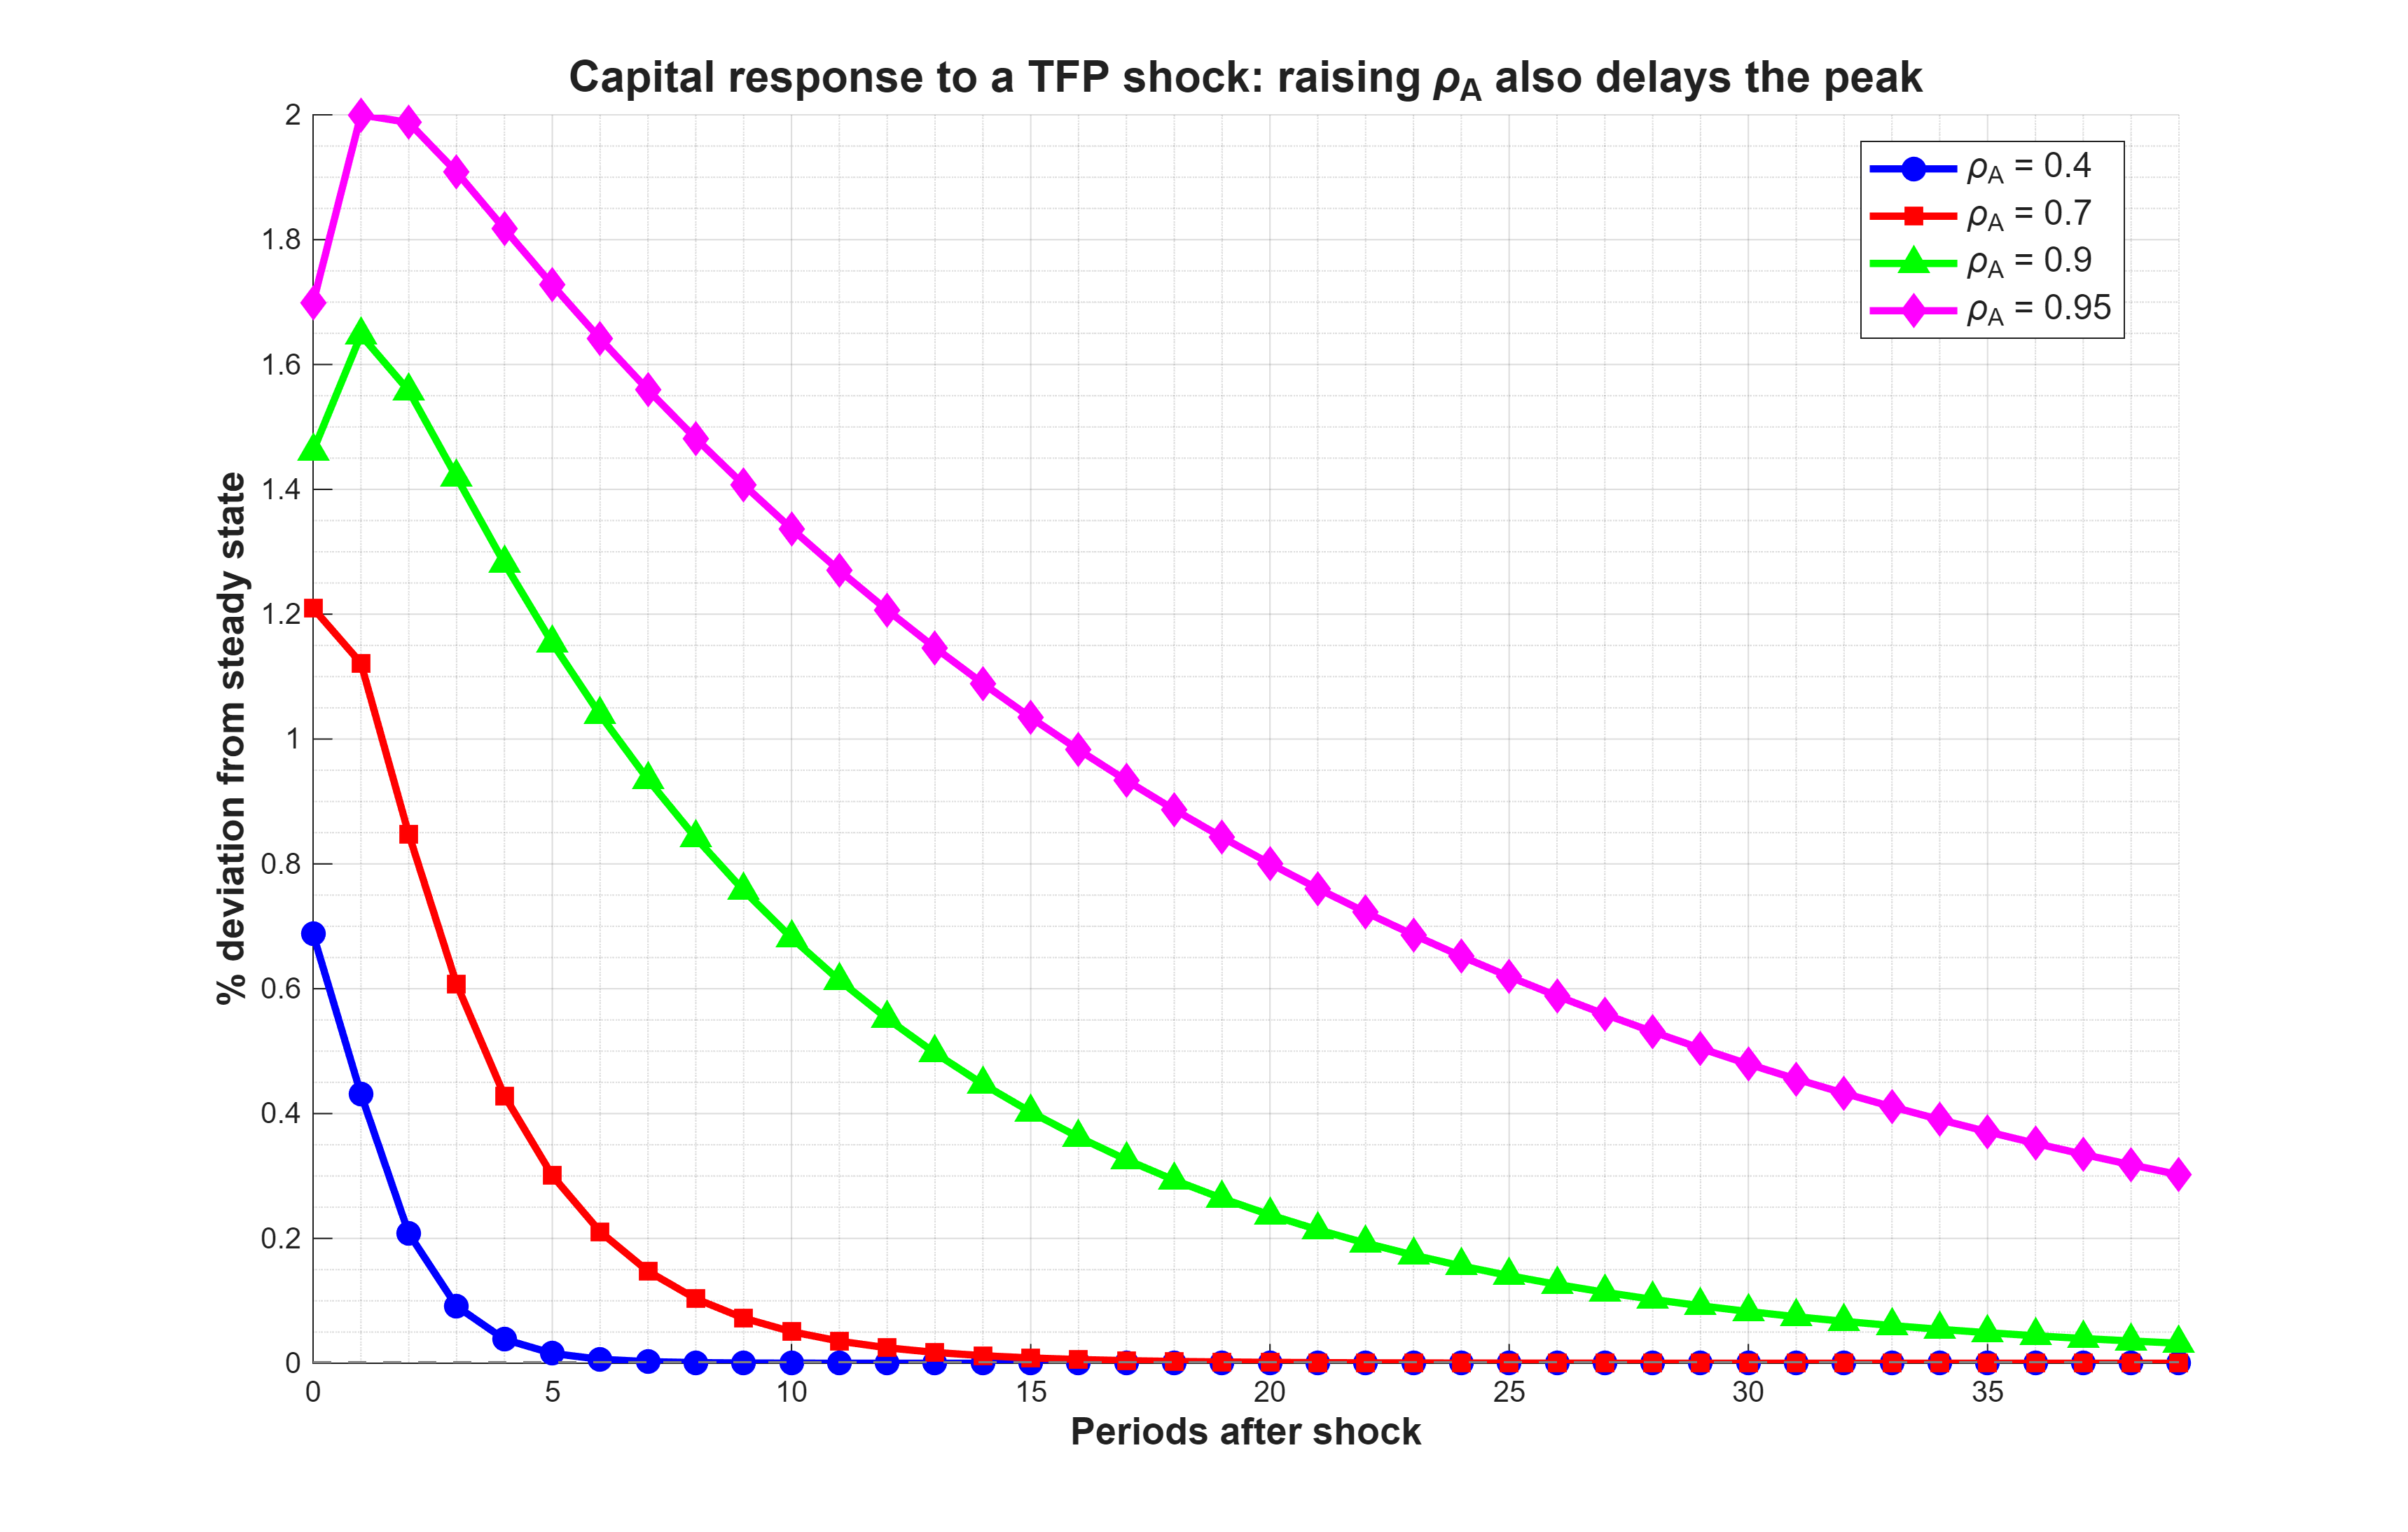
\includegraphics[width=0.78\textwidth]{q7_capital_hump_rho.png}
  \caption{Capital response to a TFP shock, by TFP persistence.}
\end{figure}

\begin{table}[h]\centering
\begin{tabular}{lcc}
\toprule
 & Peak (\% dev.) & Peak period \\
\midrule
$\phi = 0.01$   & $+0.688$ & 0 \\
$\phi = 0.5$    & $+0.079$ & 1 \\
$\phi = 2$      & $+0.026$ & 2 \\
$\phi = 6$      & $+0.010$ & 3 \\
\midrule
$\rho_A = 0.40$ & $+0.688$ & 0 \\
$\rho_A = 0.70$ & $+1.210$ & 0 \\
$\rho_A = 0.90$ & $+1.647$ & 1 \\
$\rho_A = 0.95$ & $+2.000$ & 1 \\
\bottomrule
\end{tabular}
\caption{Peak of the capital response. The $\rho_A$ block holds
$\phi = 0.01$, the $\phi$ block holds $\rho_A = 0.4$, so the first row of each
is the same baseline.}
\end{table}

\subsection*{Interpretation}

A peak at period 0 is not a hump. Both knobs produce one, but not in the same
way.

Raising $\phi$ works cleanly. The peak walks out from period 0 to 3 as $\phi$
goes from 0.01 to 6, because a quadratic adjustment cost makes one big jump
expensive relative to several small ones. The price is size: the peak falls
from $+0.69\%$ to $+0.01\%$. Capital barely moves at all, it just moves slowly.

Raising $\rho_A$ does the opposite. The peak only reaches period 1, so the hump
is mild, but the response grows from $+0.69\%$ to $+2.00\%$. Persistent TFP
keeps the incentive alive, so the firm accumulates more.

The two are different experiments. $\phi$ changes the technology of adjustment
and delays a shrinking response. $\rho_A$ changes the shock and amplifies it.
For a hump that is both late and large, raise both.


%---------------------------------------------------------------
\section{Sigma and the GHH Aggregator}

\begin{question}
Change $\sigma$ in the code, to 5 or 6, and see how $G$, the GHH consumption
aggregator, reacts. Then set it close to 1, the log case, and plot the whole
$G$ rather than consumption alone.
\end{question}

\note{File}{\texttt{dynare/q8\_ghh\_sigma.mod}, from
\texttt{GPU\_2010\_byCESG\_v110.mod}. Three lines added, each marked
\texttt{Q8}: $G$ in the \texttt{var} block, its definition, its steady state.}

\note{Where $\sigma$ is}{The file calls it \texttt{gamma}. Preferences are GHH,
\[ U = \frac{G^{1-\gamma}}{1-\gamma}, \qquad
   G = c - \frac{\theta}{\omega} h^{\omega}, \]
so \texttt{gamma} is the $\sigma$ of the question and $G$ is the whole argument
of utility. Equation 2 of the model is the marginal utility of $G$, not of $c$.}

\note{Why $G$ and not $c$}{Under GHH the labour first order condition,
$\theta h^{\omega-1} = \mathrm{MPL}$, has no consumption in it. Hours depend
only on the wage and the household smooths $G$. The gap between the $c$ path
and the $G$ path is the labour term.}

\note{Method}{Loops $\gamma \in \{1, 2, 5, 6\}$ and plots $G$ and $c$ side by
side for the transitory and the trend shock. $1/\gamma$ is the intertemporal
elasticity: at 5 or 6 the household will not move $G$ over time and the
adjustment goes to the trade balance, at 1 it moves freely.}

\subsection*{Results}

\begin{table}[h]\centering
\begin{tabular}{lcc}
\toprule
$\gamma$ & $\sigma_C/\sigma_Y$ & $\sigma_G/\sigma_Y$ \\
\midrule
1 (log) & 1.116 & 1.471 \\
2       & 1.079 & 1.291 \\
5       & 1.040 & 1.133 \\
6\,\textsuperscript{$\dagger$} & 0.729 & 1.046 \\
\bottomrule
\end{tabular}
\caption{Volatility ratios, log-linear solution, all shocks active.
\textsuperscript{$\dagger$} The solver reports
\texttt{RCOND} $\approx 10^{-16}$ at this value. See the note below.}
\end{table}

\begin{figure}[h]\centering
  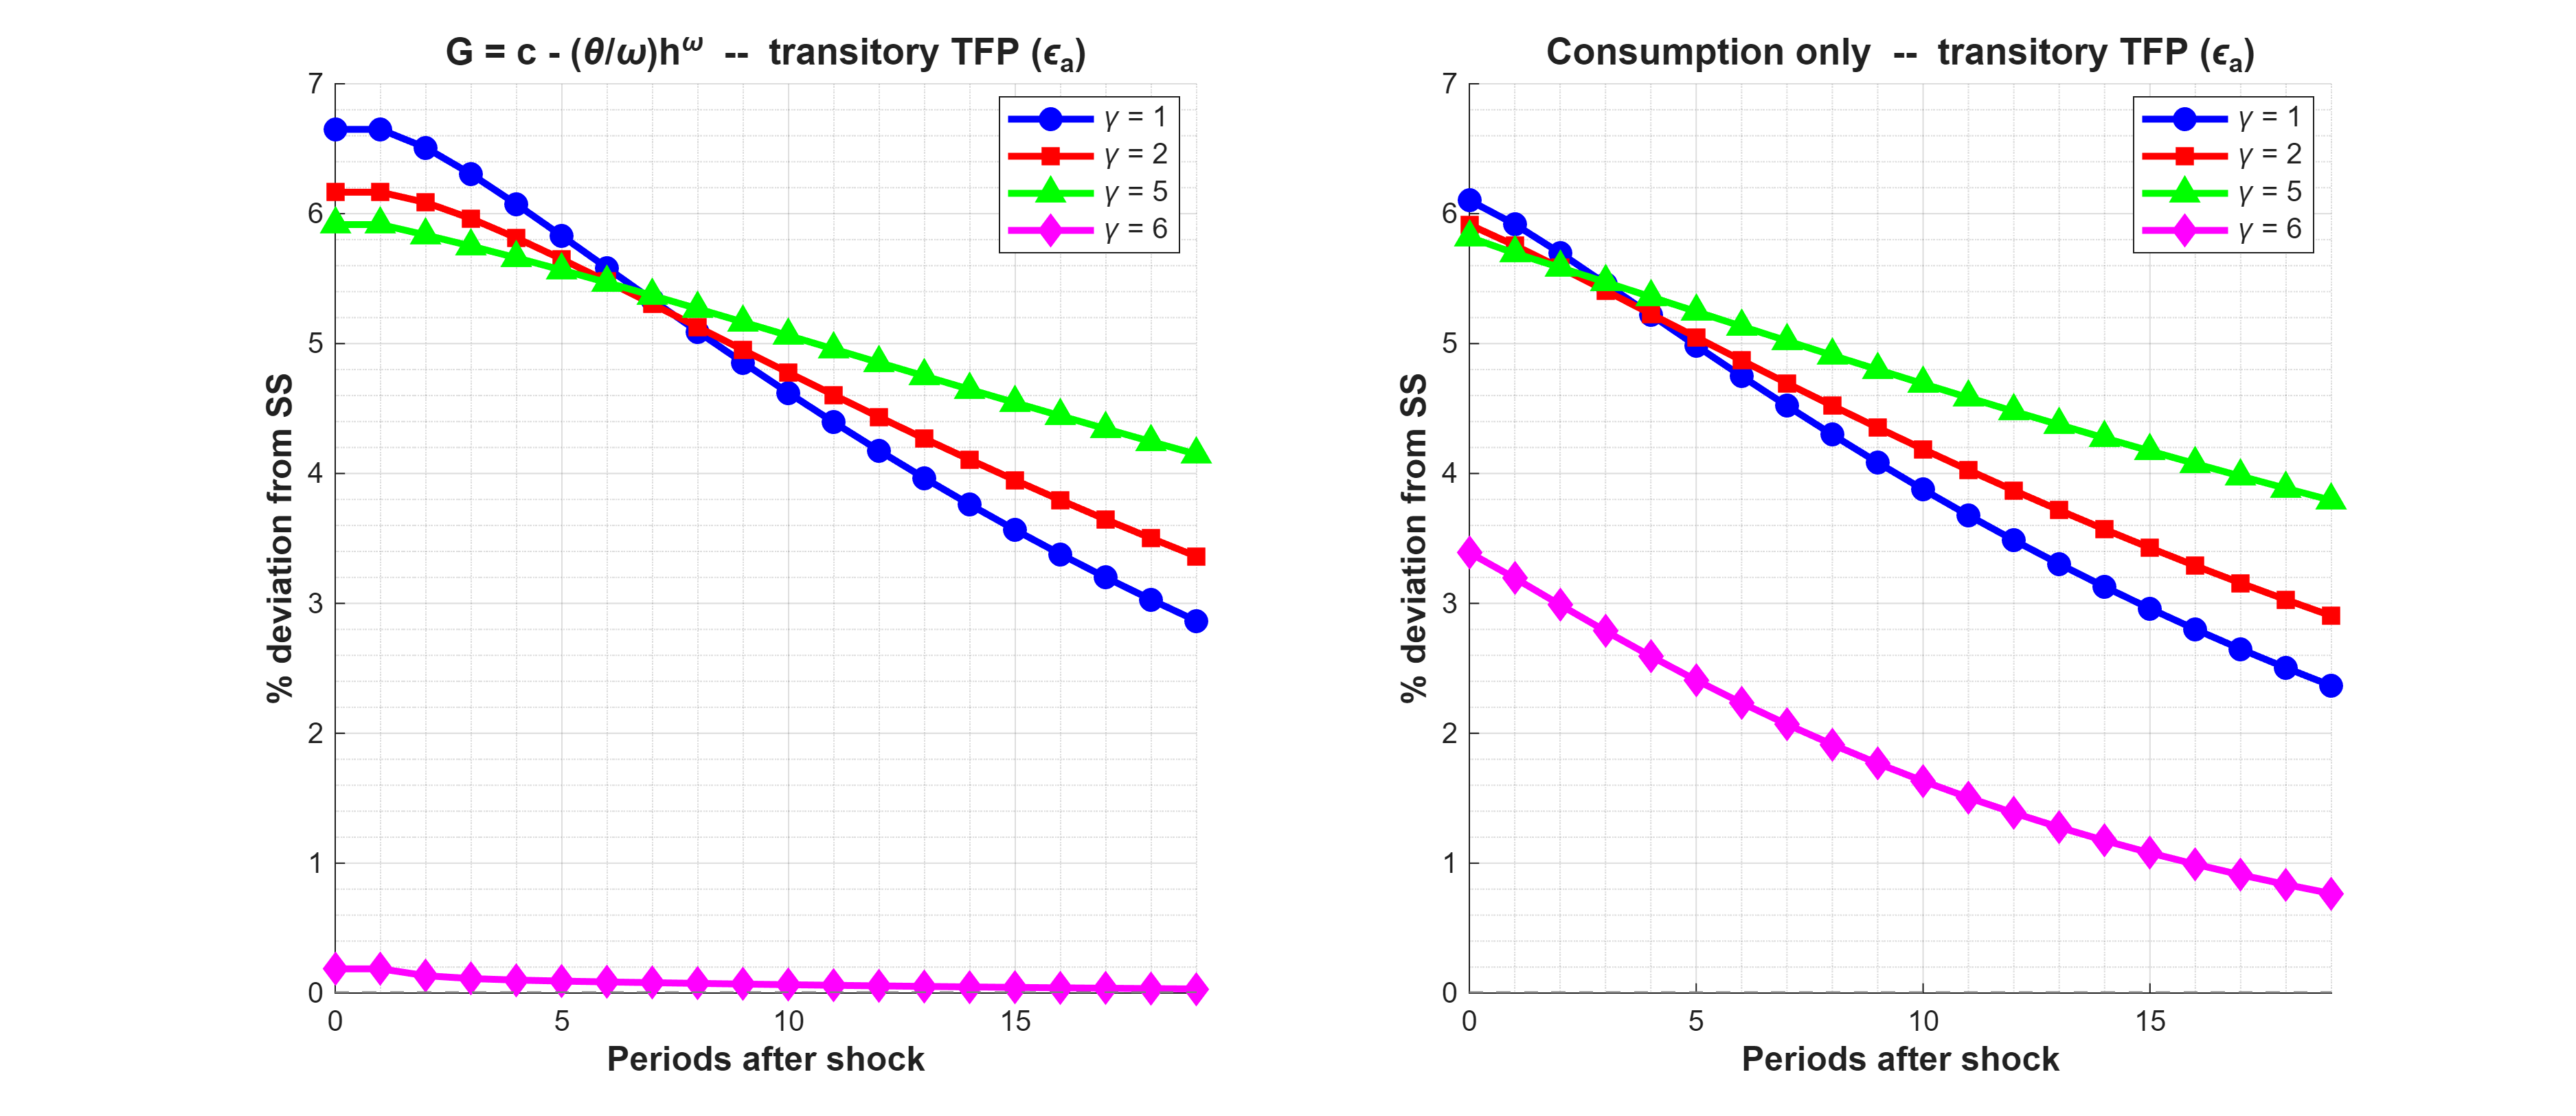
\includegraphics[width=0.95\textwidth]{q8_G_vs_c_eps_a.png}
  \caption{$G$ and $c$ after a transitory TFP shock.}
\end{figure}

\begin{figure}[h]\centering
  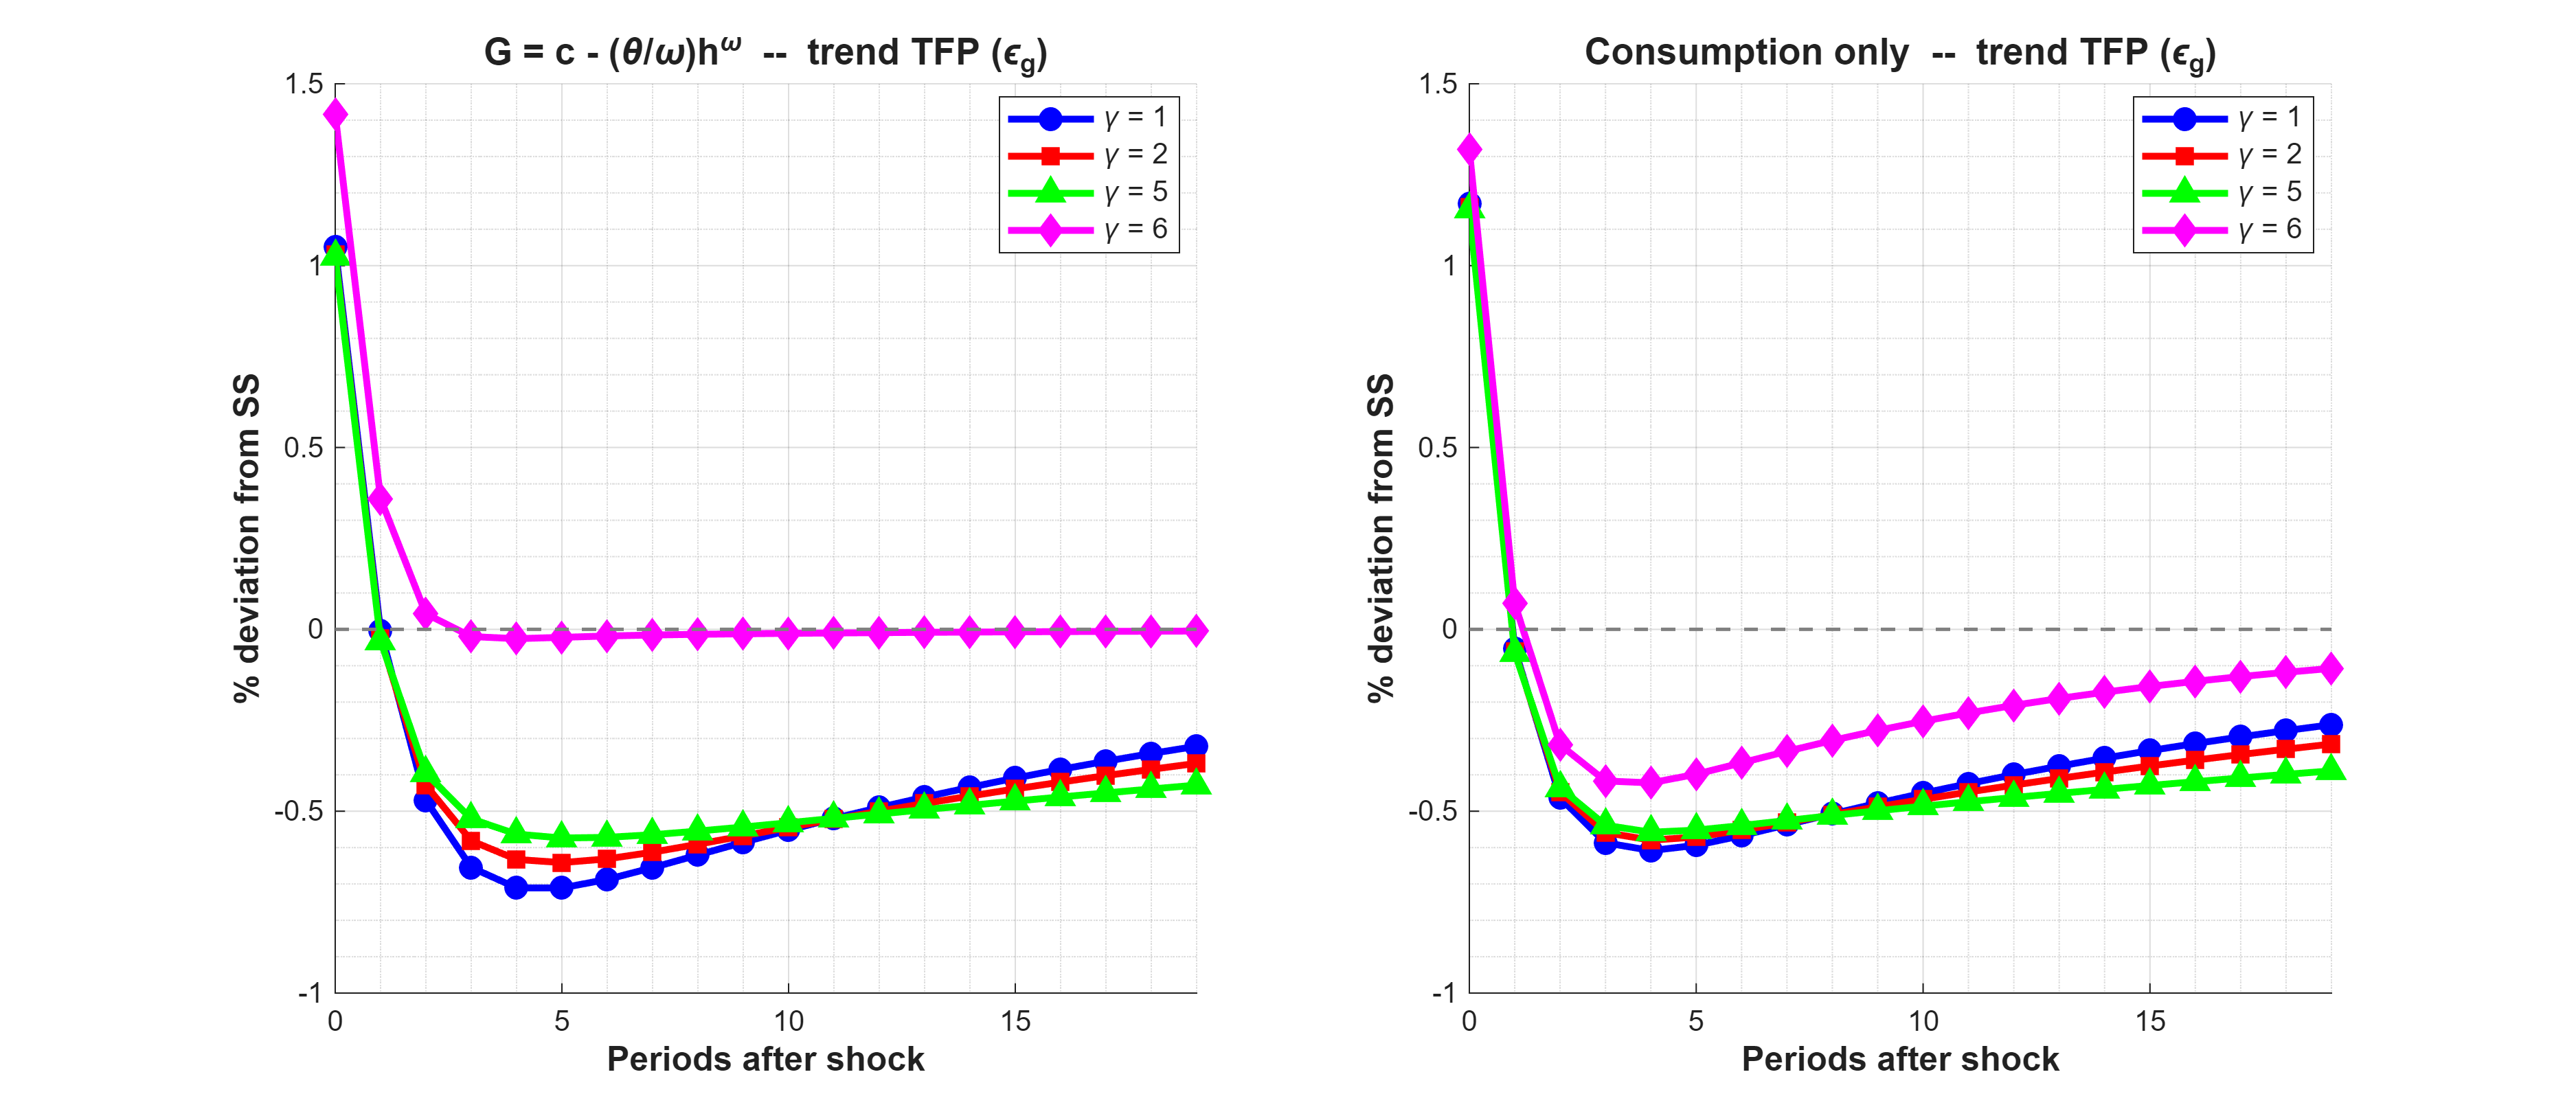
\includegraphics[width=0.95\textwidth]{q8_G_vs_c_eps_g.png}
  \caption{$G$ and $c$ after a trend TFP shock.}
\end{figure}

\subsection*{Interpretation}

$G$ is more volatile than $c$ at every $\gamma$. This is why the question asks
for $G$. Since $G = c - (\theta/\omega)h^{\omega}$ is a difference of two
positive numbers, $G < c$, and a given percentage move in $c$ is a larger
percentage move in $G$. Plotting $c$ alone understates the object inside the
utility function.

Raising $\gamma$ flattens both series. $1/\gamma$ is the intertemporal
elasticity, so a high $\gamma$ household refuses to move $G$ across time:
$\sigma_G/\sigma_Y$ goes from 1.47 at $\gamma = 1$ to 1.13 at $\gamma = 5$. The
adjustment does not vanish, it moves to the trade balance.

\medskip
\noindent\textbf{On $\gamma = 6$.} Do not use this row. The solver reports
\texttt{RCOND} $\approx 10^{-16}$, and the break is visible in the numbers:
$\sigma_G/\sigma_Y$ falls smoothly while $\sigma_C/\sigma_Y$ jumps from 1.040
to 0.729. One series breaking while its companion stays smooth is numerical,
not economic.


%---------------------------------------------------------------
\section{Persistence Close to One}

\begin{question}
Set $\rho$ close to 1 and see what happens to $\sigma_c / \sigma_y$. In the
level model, with $\rho = 0.95$, the trade balance should look like the case
with $\rho$ near 0, but return very slowly.
\end{question}

\note{File}{\texttt{dynare/q9\_rho\_near\_one.mod}, from \texttt{soe1.mod}.
Only $\rho_A$ moves, through \texttt{set\_param\_value}.}

\note{Method}{Loops $\rho_A \in \{0.05, 0.4, 0.7, 0.9, 0.95\}$. Prints
$\sigma_y$, $\sigma_c$, $\sigma_C/\sigma_Y$ and $\rho(tb/y, y)$, and plots the
$tb/y$ response over 60 periods. Moments use \texttt{hp\_filter=100} so they
match the annual empirical moments. Sigmas are coefficients of variation, which
to first order equal ratios of log standard deviations.}

\note{What to expect}{A near-permanent TFP shock raises permanent income
roughly one for one with current output, so consumption moves at least as much
and $\sigma_C/\sigma_Y$ climbs past 1. This is the Aguiar and Gopinath point:
excess consumption volatility is a statement about the income process, not
about credit constraints. Near a unit root the only force pulling debt back to
$\bar d$ is the premium $\psi = 0.01$, so the trade balance takes very long to
return.}

\note{To check}{\texttt{soe1.mod} sets
\texttt{lambda = c-(h\^{}omega)/omega}, which makes marginal utility equal to
the GHH composite itself, that is $\lambda = G^{-\sigma}$ with $\sigma = -1$.
The file also declares \texttt{sigma = 2} and never uses it. The intended line
was probably \texttt{lambda = (c-(h\^{}omega)/omega)\^{}(-sigma)}. The level of
$\sigma_C/\sigma_Y$ depends on this. The direction does not.}

\subsection*{Results}

\begin{table}[h]\centering
\begin{tabular}{lcccc}
\toprule
$\rho_A$ & $\sigma_y$ (\%) & $\sigma_c$ (\%) & $\sigma_C/\sigma_Y$ & $\rho(tb/y,\,y)$ \\
\midrule
0.05 & 1.676 & 1.009 & 0.602 & $+0.988$ \\
0.40 & 1.758 & 1.079 & 0.614 & $-0.074$ \\
0.70 & 2.081 & 1.342 & 0.645 & $-0.062$ \\
0.90 & 2.253 & 1.757 & 0.780 & $-0.085$ \\
0.95 & 2.341 & 2.177 & 0.930 & $-0.146$ \\
\bottomrule
\end{tabular}
\caption{Moments under HP(100), by TFP persistence. Sigmas are coefficients of
variation.}
\end{table}

\begin{figure}[h]\centering
  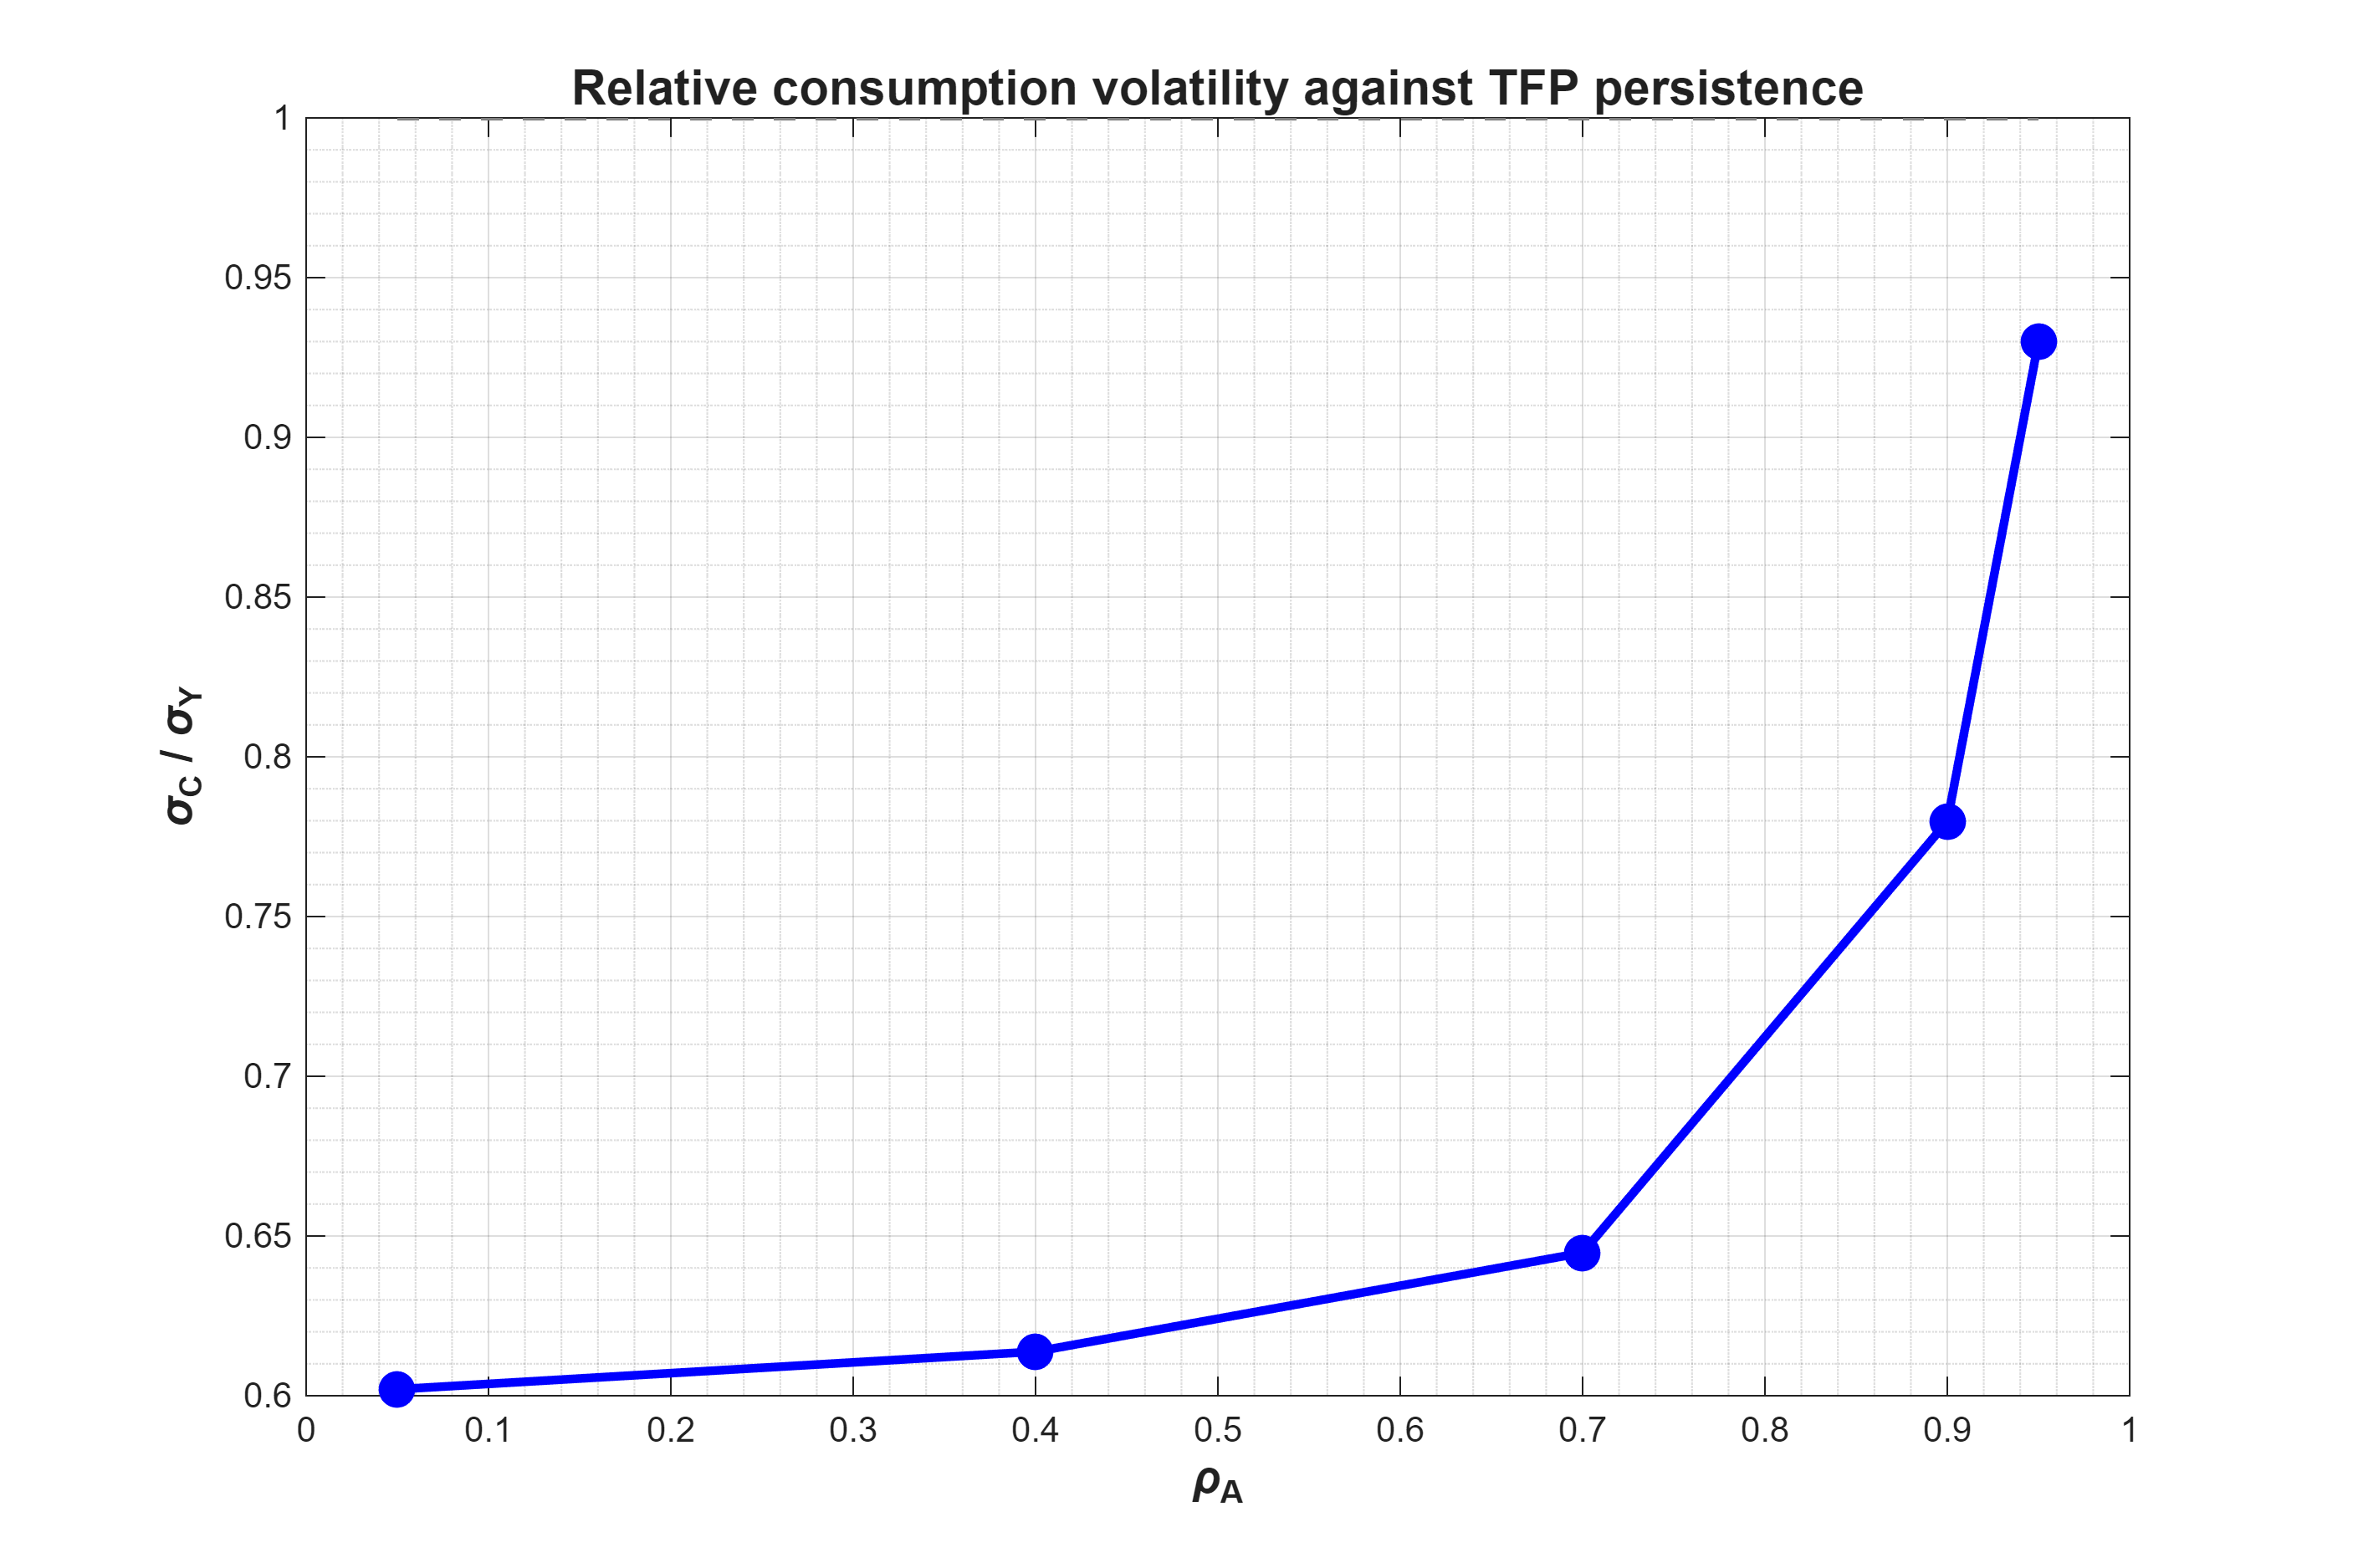
\includegraphics[width=0.78\textwidth]{q9_sigma_ratio.png}
  \caption{Relative consumption volatility against TFP persistence.}
\end{figure}

\begin{figure}[h]\centering
  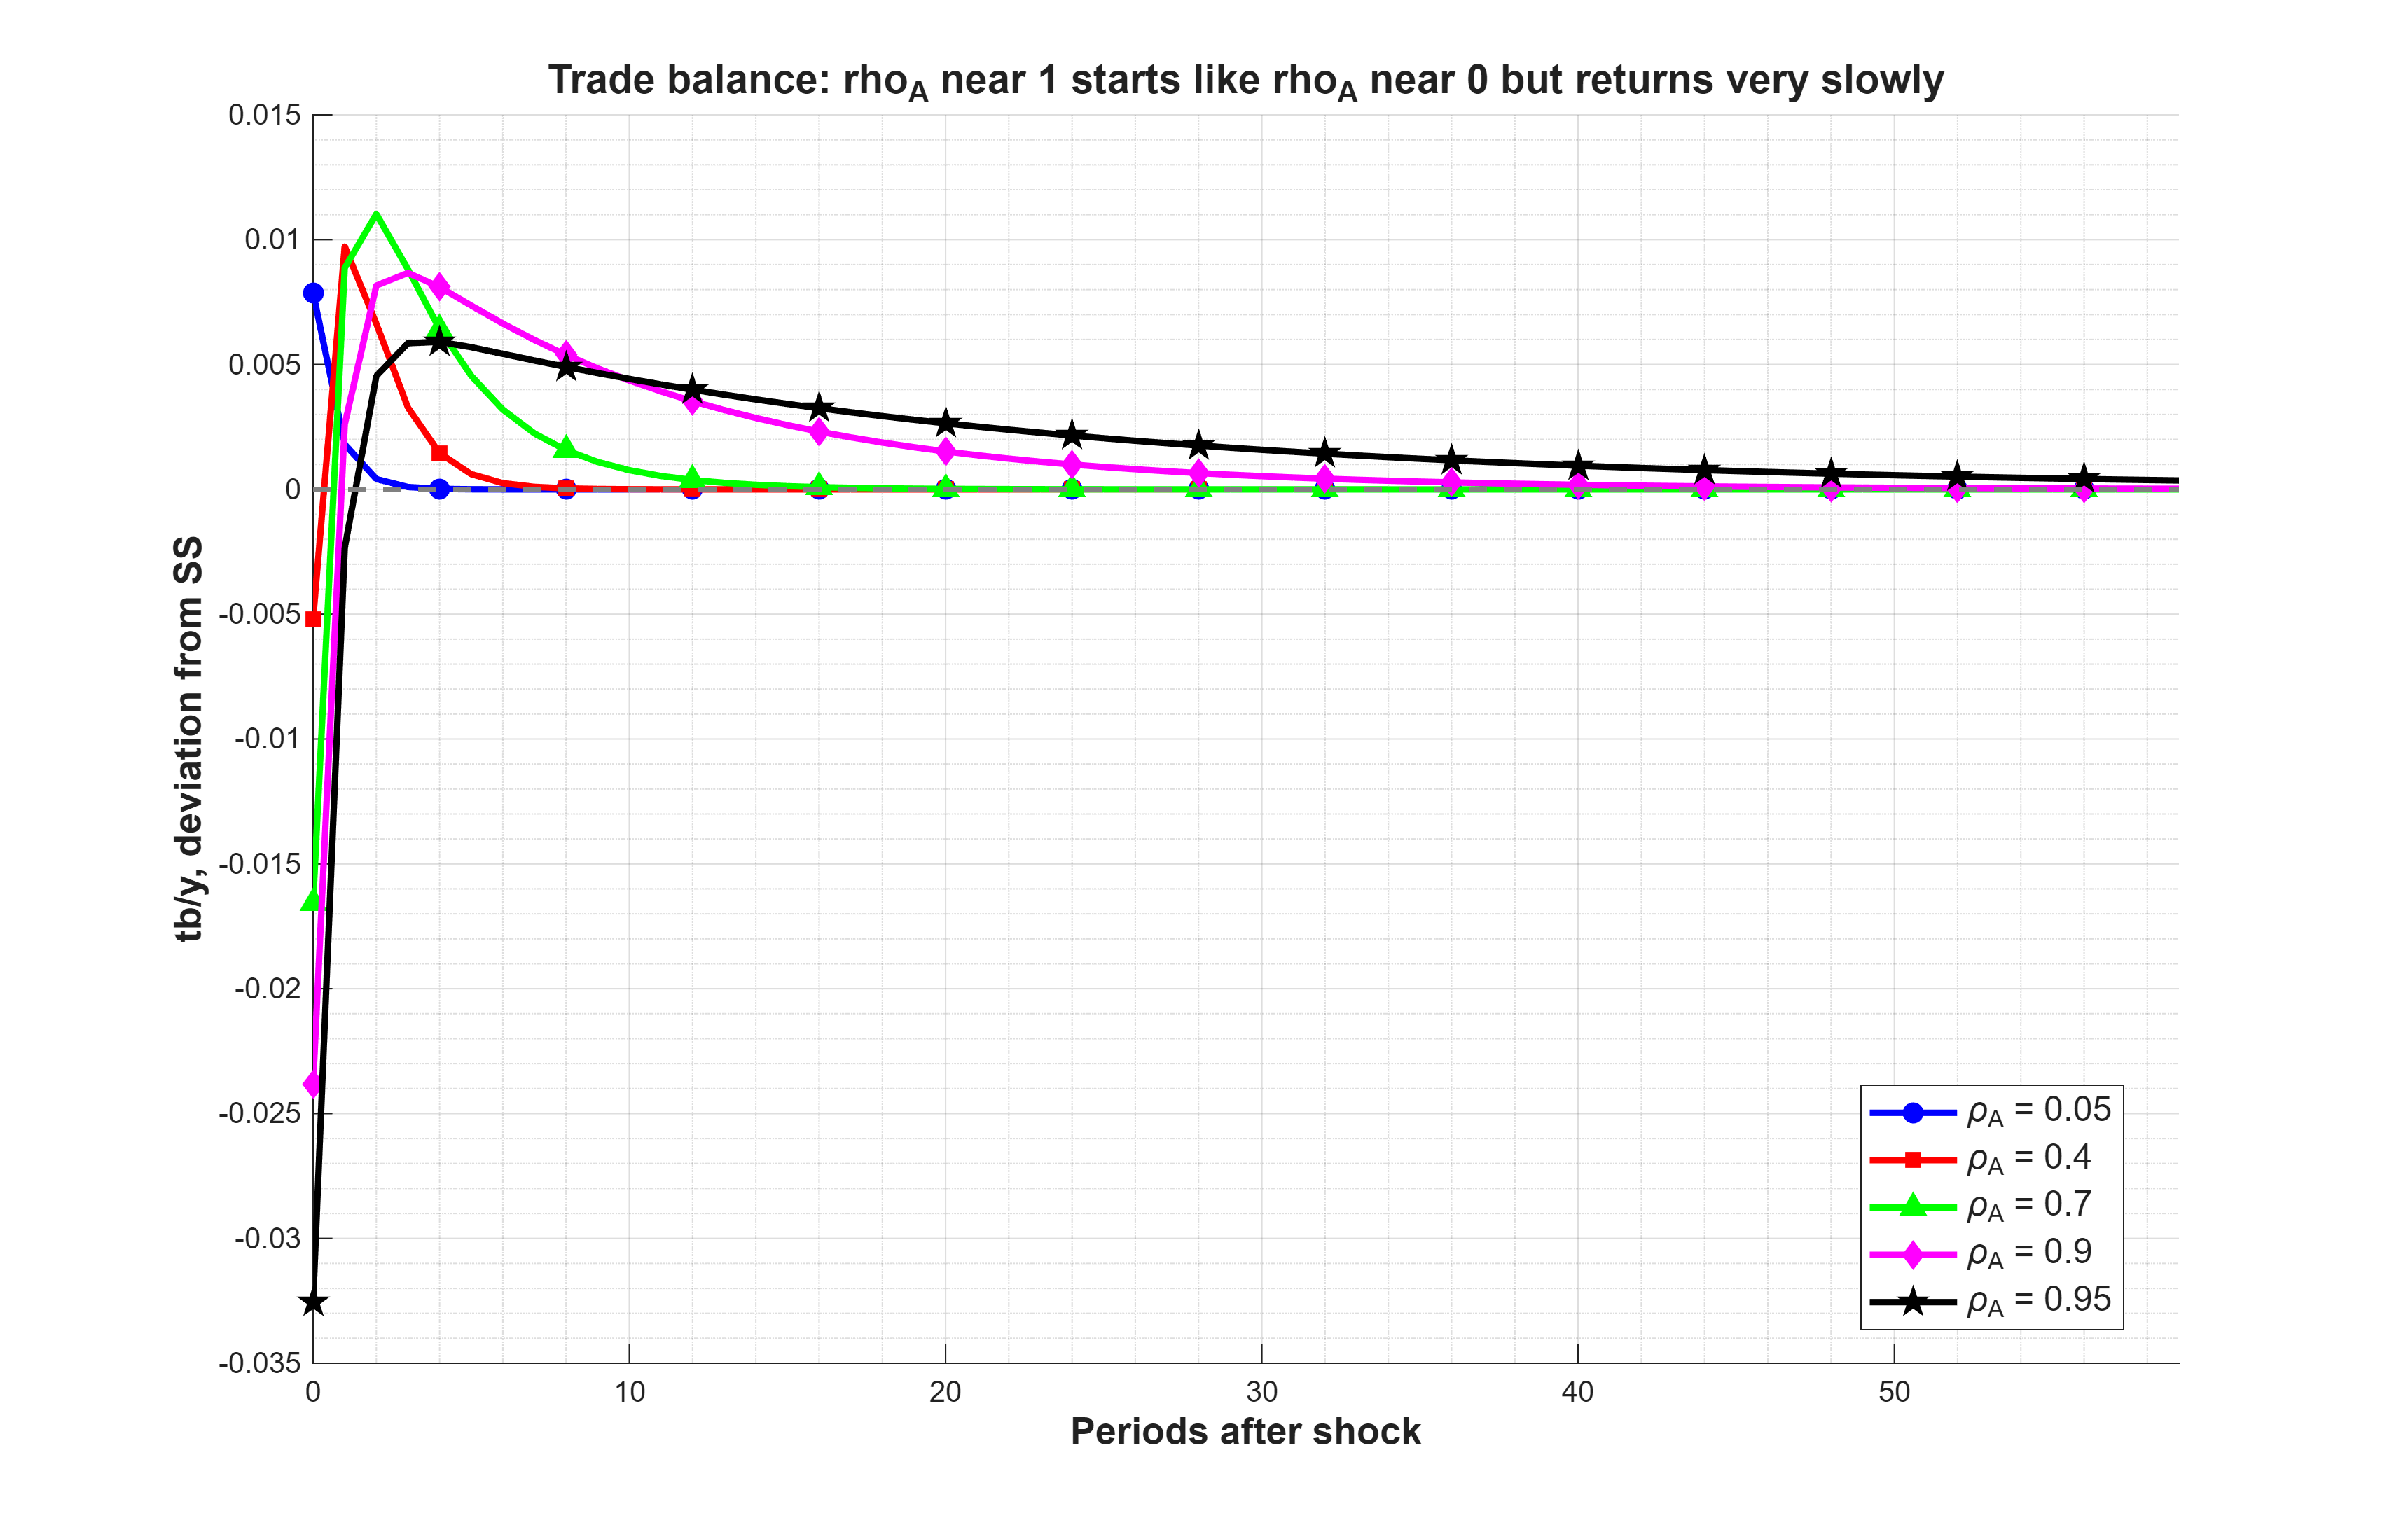
\includegraphics[width=0.78\textwidth]{q9_tb_persistence.png}
  \caption{Trade balance response, low against high persistence.}
\end{figure}

\subsection*{Interpretation}

$\sigma_C/\sigma_Y$ rises monotonically with $\rho_A$, from 0.602 to 0.930, as
predicted. A more persistent shock raises permanent income by more relative to
current income, so consumption responds by more.

It never crosses 1, and that is not a bug. This file has
$\log A_t = \rho_A \log A_{t-1} + \varepsilon_t$, an AR(1) in the \emph{level}
of TFP. The Aguiar and Gopinath mechanism needs an AR(1) in the \emph{growth
rate}. A stationary level shock raises permanent income by at most as much as
current income, so the ratio approaches 1 from below and stops.

The trade balance correlation flips from $+0.988$ to $-0.074$ between the first
two rows. At $\rho_A = 0.05$ the shock is nearly transitory, so the extra output
goes abroad and $tb/y$ is procyclical. Once it persists, consumption and
investment absorb more than the output gain and $tb/y$ turns countercyclical.
One parameter moves both moments: the deck's two facts are one fact.

The countercyclicality stays weak, $-0.06$ to $-0.15$ against the deck's
$-0.51$, for the same reason. A level shock is a weak version of the mechanism.

\medskip
\noindent\textbf{Caveat.} \texttt{soe1.mod} sets
\texttt{lambda = c-(h\^{}omega)/omega}, which makes marginal utility equal to
the GHH composite itself, and declares \texttt{sigma = 2} without using it. The
levels in the table depend on that curvature. The ranking across $\rho_A$ does
not.

\end{document}
